% 使用ctexart文档类(用XeLaTeX编译,直接支持中文)
\documentclass{standalone}

%导言区,可以在此引入必要的宏包
\usepackage{ctex}
\usepackage{tikz} % Required for drawing custom shapes
%\usetikzlibrary{arrows,calc,fit,matrix,positioning,shapes,shadows,trees,mindmap,tikzmark,arrows.meta}
\usetikzlibrary{
    decorations.markings,
    decorations.pathmorphing,
    decorations.text,
}
\usepackage{csquotes}

\begin{document} %在document环境中撰写文档

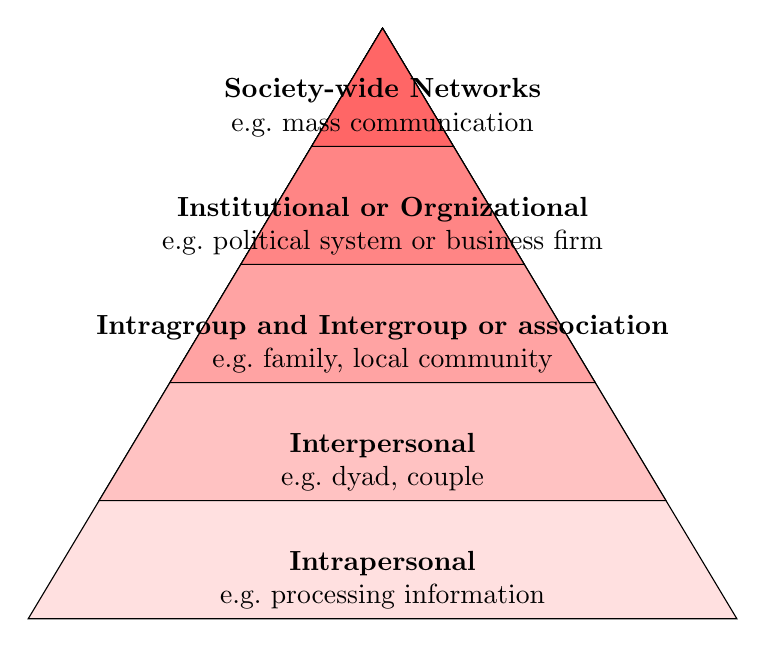
\begin{tikzpicture}[x=1.8cm,y=1.5cm]
\coordinate (A) at (-3,-1) {};
\coordinate (B) at (3,-1) {};
\coordinate (C) at (0,5) {};
\foreach \A [count=\i,evaluate=\i as \j using 12*\i] in {{\textbf{Intrapersonal}\\e.g.\ processing information}, {\textbf{Interpersonal}\\e.g.\ dyad, couple},{\textbf{Intragroup and Intergroup or association}\\e.g.\ family, local community},{\textbf{Institutional or Orgnizational}\\e.g.\ political system or business firm},{\textbf{Society-wide Networks}\\e.g.\ mass communication}}
\draw[fill=red!\j] (C)--([shift={(-.5*\i,1*\i)}]B)--node[above,align=center] {\A}([shift={(.5*\i,1*\i)}]A)--cycle;
\end{tikzpicture}

\end{document}



%%% Local Variables:
%%% mode: latex
%%% TeX-master: t
%%% End:
